\subsection{Background}

In today's connected digital world, cryptographic algorithms are implemented in every device and applied to every link to protect information in transmission and in storage.
Data security is a challenging issue that covers many areas including computer and communication.
There has been a rise of cyber attacks in gaining access to computers or computer networks, to gain information of private and sensitive data to gain information via communication channels or unsecure files \cite{csis2025significant}. 

Cryptology is the science of devising methods that allow information to be sent in a secure form in such a way that the only person able to retrieve the information is the recipient, through the use of algorithms. 
Data is exchanged while communicating from one system to another through the use of networks. 
It is important to encrypt the message so that unintended recipients (intruders) are unable to read the message as network security is highly based on cryptology.
Essentially, cryptography is the art of protecting information through encryption into an unreadable format, i.e. encrypted text or cipher text. 
Only those who posses a secret key can decipher (decrypt) the message back into plain text \cite{Bhanot_2015}. 
Figure \ref{fig:encryption-process.png} describes the encryption and decryption process. 

\begin{figure}[h]
    \centering
    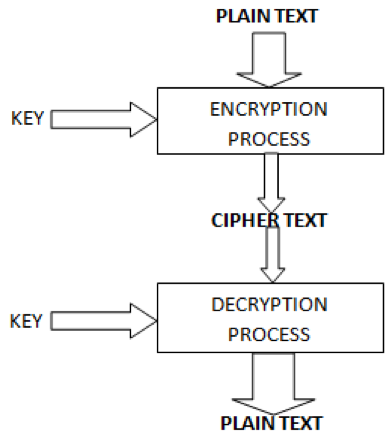
\includegraphics[width=.35\textwidth]{encryption-process.png}
    \caption{Encryption and decryption process \cite{Bhanot_2015}.}
    \label{fig:encryption-process.png}
\end{figure}

Over the past 50 years, the use of cryptographic tools have expanded dramatically, from limited environments like \gls{ATM} encryption to every digital application used today. 
\Gls{NIST} has played a unique leading role in developing critical standards \cite{chen2022cornerstone}:
\begin{itemize}
    \item \textbf{\Gls{DES}}: Developed in 1973 to protect computer data to allow for large-scale interoperability. \Gls{DES} uses a 64-bit block cipher with 56-bit key.
    \item \textbf{\Gls{AES}}: Developed in 1997 to superceeded \gls{DES}, with the use of 128-bit block cipher with three key length options: 128, 192, and 256 bits. 
    \item \textbf{Public-Key Cryptology}: Invented in 1976 to allow different parties to establish keys without protected channel and enabling the function of digital signatures. 
    \item \textbf{\Gls{PQC}}: Begun development in 2016 to develop quantum-resistant cryptography standards (i.e., \gls{PQC}) to provide security protection against quantum computers. As of writing this paper, \gls{NIST} have released the first three finalised Post-Quantum Encryption Standards \cite{nist2024postquantum}.
\end{itemize}

